\documentclass{article}
\usepackage[utf8]{inputenc}
\usepackage[brazil]{babel}
\usepackage{mathtools}
\usepackage{wrapfig}
\usepackage{graphicx}
\usepackage[colorlinks, linkcolor=blue, urlcolor=blue, citecolor=blue]{hyperref}
\usepackage[a4paper, left=20mm, right=20mm, top=20mm, bottom=20mm]{geometry}

\title{\textbf{AES: Advanced Encryption Standard \\
        \large INE5429 - Segurança em Computação}}
\author{
    Caique Rodrigues Marques \\
    {\texttt{c.r.marques@grad.ufsc.br}}
}
\date{}

\begin{document}

\maketitle

\section{AES Simplificado}
\subsection{Cifração}
A entrada $t$ para o AES corresponde ao número do dia do aniversário acrescido
de 10000, portanto, $10000 + 25 = 10025$. A chave $k$ é o número do aniversário
somado a 8000, portanto, $8000 + 25 = 8025$. Em hexadecimal, temos que $t =$
\texttt{2729} e $k =$ \texttt{1F59}.
\begin{enumerate}
    \item \textbf{Incluir chave de rodada}: Esta função apenas consiste na
    operação de ou-exclusivo (XOR) de 16 bits entre a entrada $t$ com a chave
    $k$. Abaixo está representada em tabelas a operação realizada:
    \begin{center}
        \begin{tabular}{|c|c|}
            \hline
            2 & 2  \\
            \hline
            7 & 9 \\
            \hline
        \end{tabular}
        $\oplus$
        \begin{tabular}{|c|c|}
            \hline
            1 & 5  \\
            \hline
            F & 9 \\
            \hline
        \end{tabular}
        $=$
        \begin{tabular}{|c|c|}
            \hline
            3 & 7  \\
            \hline
            8 & 0 \\
            \hline
        \end{tabular}
    \end{center}
    \begin{gather*}
        2 \oplus 1 = 0010 \oplus 0001 = 3 \\
        7 \oplus F = 0111 \oplus 1111 = 8 \\
        2 \oplus 5 = 0010 \oplus 0101 = 7 \\
        9 \oplus 9 = 1001 \oplus 1001 = 0 \\
    \end{gather*}
    
    \item \textbf{Substituir \textit{nibble}}: A função de substituição do
    \textit{nibble} é apenas uma pesquisa em uma tabela. O AES define uma
    matriz 4x4 dos valores de \textit{nibbles}, chamada de \textit{S-box}, que
    consiste em uma permutação de todos os possíveis valores de 4 bits. Cada
    \textit{nibble} da entrada é mapeada para o novo \textit{nibble} definido
    na \textit{S-box} da seguinte maneira: os dois bits mais à esquerda
    correspondem à linha da \textit{S-box}, enquanto os dois bits mais à
    direita correspondem à coluna da \textit{S-box}. Por exemplo, o valor
    hexadecimal \texttt{8}, em binário é $1000$, é mapeado para a linha 2 e
    coluna 0 da S-box, que resulta no valor \texttt{6}. A seguir, à esquerda
    está a \textit{S-box}, enquanto à direita está a substituição dos
    \textit{nibbles} da saída do passo anterior.

    \begin{minipage}{0.32\textwidth}
        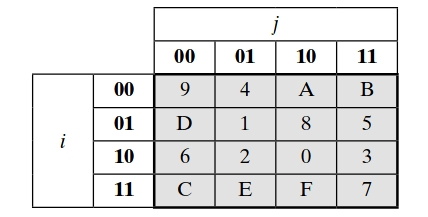
\includegraphics[width=\linewidth]{imgs/s-box.jpg}
    \end{minipage}
    \begin{minipage}{0.6\textwidth}
        \begin{tabular}{|c|c|}
            \hline
            3 & 7  \\
            \hline
            8 & 0 \\
            \hline
        \end{tabular}
        $\to$
        \begin{tabular}{|c|c|}
            \hline
            B & 5  \\
            \hline
            6 & 9 \\
            \hline
        \end{tabular}
    \end{minipage}

    \item \textbf{Deslocar linhas}: A função de deslocar linhas realiza uma
    rotação circular de um \textit{nibble} da segunda linha, enquanto a
    primeira linha permanece inalterada, assim:
    \begin{center}
        \begin{tabular}{|c|c|}
            \hline
            B & 5  \\
            \hline
            6 & 9 \\
            \hline
        \end{tabular}
        $\to$
        \begin{tabular}{|c|c|}
            \hline
            B & 5  \\
            \hline
            9 & 6 \\
            \hline
        \end{tabular}
    \end{center}
    
    \item \textbf{Embaralhar colunas}: A transformação pode ser definida pelas
    seguintes operações, onde o operador $\cdot$ corresponde à multiplicação em
    $GF(2^{4})$.
    \begin{center}
        \begin{gather*}
            S'_{0, 0} = (B \cdot 1) \oplus (4 \cdot 9) = B \oplus 2 = 9 \\
            S'_{1, 0} = (B \cdot 4) \oplus (1 \cdot 9) = A \oplus 9 = 3 \\
            S'_{0, 1} = (5 \cdot 1) \oplus (4 \cdot 6) = 5 \oplus B = E \\
            S'_{1, 1} = (5 \cdot 4) \oplus (1 \cdot 6) = 7 \oplus 6 = 1
        \end{gather*}
    \end{center}
    
    \item \textbf{Expansão da chave}: O algoritmo de expansão é definido a
    seguir, onde, da chave $k$, temos $w_{0} =$ \texttt{1F} e $w_{1} = 59$;
    \texttt{RotNib} corresponde à rotação circular à esquerda de um
    \textit{nibble}; \texttt{SubNib} refere-se aos \textit{nibbles}
    correspondentes na \textit{S-box}. A partir da chave $k$ de 16 bits, ela é
    expandida para seis palavras de 8 bits cada uma.

    $w_{2} = w_{0} \oplus g(w_{1})$ \\
    $= w_{0} \oplus Rcon(1) \oplus SubNib(RotNib(w_{1}))$ \\
    $= 00011111 \oplus 10000000 \oplus SubNib(10010101)$ \\
    $= 00011111 \oplus 10000000 \oplus 00100001 = 10111110$
    
    $w_{3} = w_{2} \oplus w_{1} = 10111110 \oplus 01011001 = 11100111$
    
    $w_{4} = w_{2} \oplus g(w_{3})$ \\
    $= w_{2} \oplus Rcon(2) \oplus SubNib(RotNib(w_{3}))$ \\
    $= 10111110 \oplus 00110000 \oplus SubNib(01111110)$ \\
    $= 10111110 \oplus 00110000 \oplus 01011111 = 11010001$
    
    $w_{5} = w_{4} \oplus w_{3} = 11010001 \oplus 11100111 = 00110110$
    
    \item \textbf{Incluir chave de rodada}: Operação de ou-exclusivo entre o
    resultado do embaralhamento de colunas (passo 4) e a concatenação de
    $w_{2}$ e $w_{3}$, do passo anterior:
    
    \begin{center}
        \begin{tabular}{|c|c|}
            \hline
            9 & E  \\
            \hline
            3 & 1 \\
            \hline
        \end{tabular}
        $\oplus$
        \begin{tabular}{|c|c|}
            \hline
            B & E  \\
            \hline
            E & 7 \\
            \hline
        \end{tabular}
        $=$
        \begin{tabular}{|c|c|}
            \hline
            2 & 0  \\
            \hline
            D & 6 \\
            \hline
        \end{tabular}
    \end{center}
    \begin{gather*}
        9 \oplus B = 1001 \oplus 1011 = 2 \\
        3 \oplus E = 0011 \oplus 1110 = D \\
        E \oplus E = 1110 \oplus 1110 = 0 \\
        1 \oplus 7 = 0001 \oplus 0111 = 6
    \end{gather*}
    
    \item \textbf{Substituir \textit{nibble}}:Mesmo procedimento realizado no
    passo 2, o resultado do passo anterior é associado à \textit{S-box}.
    \begin{center}
        \begin{tabular}{|c|c|}
            \hline
            2 & 0  \\
            \hline
            D & 6 \\
            \hline
        \end{tabular}
        $\to$
        \begin{tabular}{|c|c|}
            \hline
            A & 9  \\
            \hline
            E & 8 \\
            \hline
        \end{tabular}
    \end{center}
    
    \item \textbf{Deslocar linhas}: Similar ao passo 3.
    \begin{center}
        \begin{tabular}{|c|c|}
            \hline
            A & 9  \\
            \hline
            E & 8 \\
            \hline
        \end{tabular}
        $\to$
        \begin{tabular}{|c|c|}
            \hline
            A & 9  \\
            \hline
            8 & E \\
            \hline
        \end{tabular}
    \end{center}
    
    \item \textbf{Incluir chave de rodada}: Similar ao passo 1. A operação de
    ou-exclusivo é realizada entre o resultado do passo anterior com a
    concatenação das palavras $w_{4}$ e $w_{5}$ do passo 5.
        \begin{center}
        \begin{tabular}{|c|c|}
            \hline
            A & 9  \\
            \hline
            8 & E \\
            \hline
        \end{tabular}
        $\oplus$
        \begin{tabular}{|c|c|}
            \hline
            D & 3  \\
            \hline
            1 & 6 \\
            \hline
        \end{tabular}
        $=$
        \begin{tabular}{|c|c|}
            \hline
            7 & A  \\
            \hline
            9 & 8 \\
            \hline
        \end{tabular}
    \end{center}
\end{enumerate}
Assim, o texto cifrado $c$ resultante é \texttt{79A8}.

\subsection{Decifração}
A entrada para o AES é o resultado da cifragem, realizada anteriormente, que é
\texttt{727A}.
\begin{enumerate}
    \item \textbf{Incluir chave de rodada}: Esta função apenas consiste na
    operação de ou-exclusivo (XOR) de 16 bits entre a entrada com a
    concatenação das palavras $w_{4}$ e $w_{5}$ (ver passo 5 da subseção de
    cifragem). Abaixo está representada em tabelas a operação realizada:
    \begin{center}
        \begin{tabular}{|c|c|}
            \hline
            7 & A  \\
            \hline
            9 & 8 \\
            \hline
        \end{tabular}
        $\oplus$
        \begin{tabular}{|c|c|}
            \hline
            D & 3  \\
            \hline
            1 & 6 \\
            \hline
        \end{tabular}
        $=$
        \begin{tabular}{|c|c|}
            \hline
            A & 9  \\
            \hline
            8 & E \\
            \hline
        \end{tabular}
    \end{center}
    
    \item \textbf{Deslocar linhas invertidas}: A função de deslocar linhas
    realiza uma rotação circular de um \textit{nibble} da segunda linha,
    enquanto a primeira linha permanece inalterada, assim:
    \begin{center}
        \begin{tabular}{|c|c|}
            \hline
            A & 9  \\
            \hline
            8 & E \\
            \hline
        \end{tabular}
        $\to$
        \begin{tabular}{|c|c|}
            \hline
            A & 9  \\
            \hline
            E & 8 \\
            \hline
        \end{tabular}
    \end{center}
    
    \item \textbf{Substituir \textit{nibble} invertido}: A função realiza o
    inverso da \textit{S-box} (ver tabela na parte 2 da seção de cifragem),
    resultando na tabela \textit{S-box} invertido. A seguir, à esquerda está a
    \textit{S-box} invertido, enquanto à direita está a substituição dos
    \textit{nibbles} da saída do passo anterior.

    \begin{minipage}{0.32\textwidth}
        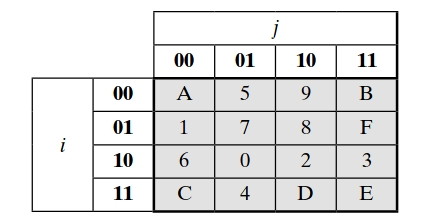
\includegraphics[width=\linewidth]{imgs/inverse_s-box.jpg}
    \end{minipage}
    \begin{minipage}{0.6\textwidth}
        \begin{tabular}{|c|c|}
            \hline
            A & 9  \\
            \hline
            E & 8 \\
            \hline
        \end{tabular}
        $\to$
        \begin{tabular}{|c|c|}
            \hline
            2 & 0 \\
            \hline
            D & 6 \\
            \hline
        \end{tabular}
    \end{minipage}
    
    \item \textbf{Incluir chave de rodada}: Esta função apenas consiste na
    operação de ou-exclusivo (XOR) de 16 bits entre a saída do passo anterior
    com a concatenação das palavras $w_{2}$ e $w_{3}$ (ver passo 5 da subseção
    de cifragem). Abaixo está representada em tabelas a operação realizada:
    \begin{center}
        \begin{tabular}{|c|c|}
            \hline
            2 & 0  \\
            \hline
            D & 6 \\
            \hline
        \end{tabular}
        $\oplus$
        \begin{tabular}{|c|c|}
            \hline
            B & E  \\
            \hline
            E & 7 \\
            \hline
        \end{tabular}
        $=$
        \begin{tabular}{|c|c|}
            \hline
            9 & E  \\
            \hline
            3 & 1 \\
            \hline
        \end{tabular}
    \end{center}
    
    \item \textbf{Embaralhar colunas invertidas}: A transformação pode ser
    definida pelas seguintes operações, onde o operador $\cdot$ corresponde à
    multiplicação em $GF(2^{4})$.
    \begin{center}
        \begin{gather*}
            S'_{0,0} = (9 \cdot 9) \oplus (2 \cdot 3) = D \oplus 6 = B \\
            S'_{1,0} = (2 \cdot 9) \oplus (9 \cdot 3) = 1 \oplus 8 = 9 \\
            S'_{0,1} = (9 \cdot E) \oplus (2 \cdot 1) = 7 \oplus 2 = 5 \\
            S'_{1,1} = (2 \cdot E) \oplus (9 \cdot 1) = F \oplus 9 = 6
        \end{gather*}
    \end{center}
    
    \item \textbf{Deslocar linhas invertidas}: A função de deslocar linhas
    realiza uma rotação circular de um \textit{nibble} da segunda linha,
    enquanto a primeira linha permanece inalterada, assim:
    \begin{center}
        \begin{tabular}{|c|c|}
            \hline
            B & 5  \\
            \hline
            9 & 6 \\
            \hline
        \end{tabular}
        $\to$
        \begin{tabular}{|c|c|}
            \hline
            B & 5  \\
            \hline
            6 & 9 \\
            \hline
        \end{tabular}
    \end{center}
    
    \item \textbf{Substituir \textit{nibble} invertido}: Similar ao passo 3 da
    decifragem.
    \begin{center}
        \begin{tabular}{|c|c|}
            \hline
            B & 5  \\
            \hline
            6 & 9 \\
            \hline
        \end{tabular}
        $\to$
        \begin{tabular}{|c|c|}
            \hline
            3 & 7  \\
            \hline
            8 & 0 \\
            \hline
        \end{tabular}
    \end{center}
    
    \item \textbf{Incluir chave de rodada}: Esta função apenas consiste na
    operação de ou-exclusivo (XOR) de 16 bits entre a saída do passo anterior
    com a chave $k$. Abaixo está representada em tabelas a operação realizada:
    \begin{center}
        \begin{tabular}{|c|c|}
            \hline
            3 & 7 \\
            \hline
            8 & 0 \\
            \hline
        \end{tabular}
        $\oplus$
        \begin{tabular}{|c|c|}
            \hline
            1 & 5 \\
            \hline
            F & 9 \\
            \hline
        \end{tabular}
        $=$
        \begin{tabular}{|c|c|}
            \hline
            2 & 2  \\
            \hline
            7 & 9 \\
            \hline
        \end{tabular}
    \end{center}
\end{enumerate}
Assim o texto original $t$ resultante é \texttt{2729}.

\section{AES Padrão}
\subsection{Cifração}
O AES padrão exige que a chave tenha pelo menos 128 bits, então, para resolver
o problema, é realizado um \textit{padding} à esquerda com zeros. Assim os
valores passam a ser os indicados na tabela abaixo. Os dez rounds de cifração
estão indicados na tabela \ref{fig:tab1} - o resultado está indicado na última
linha, na coluna \texttt{AddRoundKey}.
\begin{center}
    \begin{tabular}{|c|c|}
        \hline
        Texto original: & \texttt{00000000000000000000000000002729} \\
        \hline
        Chave: & \texttt{00000000000000000000000000001F59} \\
        \hline
        Texto cifrado: & \texttt{33A0A57199C5876778EA7B2C56970774} \\
        \hline
    \end{tabular}
\end{center}

\subsection{Decifração}
A saída da cifragem é usada como entrada para o decifrador AES padrão. A chave
$k$ possui 16 bits, assim, foi realizado um \textit{padding} à esquerda com
zeros, até completar 128 bits. Os valores finais estão indicados na tabela
abaixo. Os dez rounds de decifração estão indicados na tabela \ref{fig:tab2} -
a saída está apresentada na primeira linha, na coluna \texttt{AddRoundKey}.
\begin{center}
    \begin{tabular}{|c|c|}
        \hline
        Texto cifrado & \texttt{33A0A57199C5876778EA7B2C56970774} \\
        \hline
        Chave & \texttt{00000000000000000000000000001F59} \\
        \hline
        Texto original & \texttt{00000000000000000000000000002729} \\
        \hline
    \end{tabular}
\end{center}

\begin{figure}
    \centering
    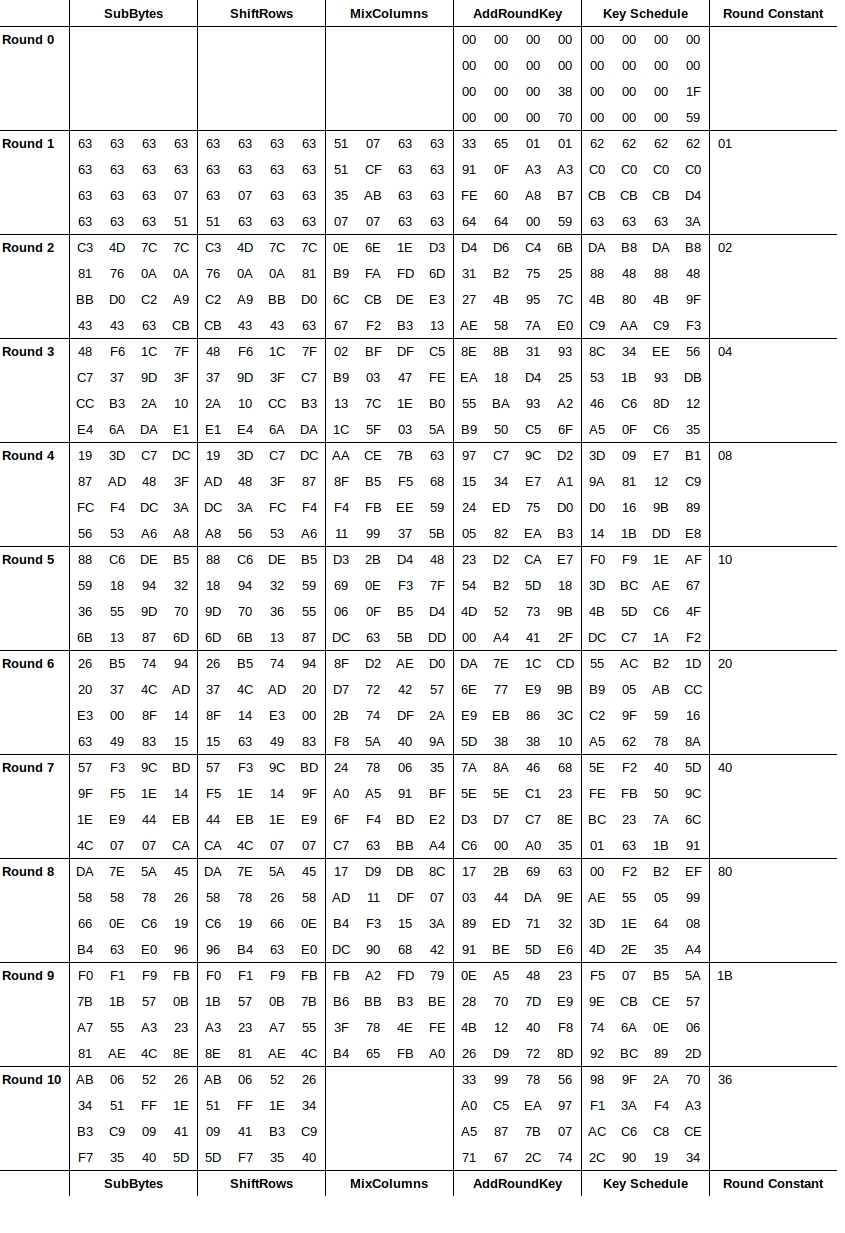
\includegraphics[width=1\linewidth]{imgs/table_aes_ciph.jpg}
    \caption{Tabela com 10 rounds de cifração.}
    \label{fig:tab1}
\end{figure}

\begin{figure}
    \centering
    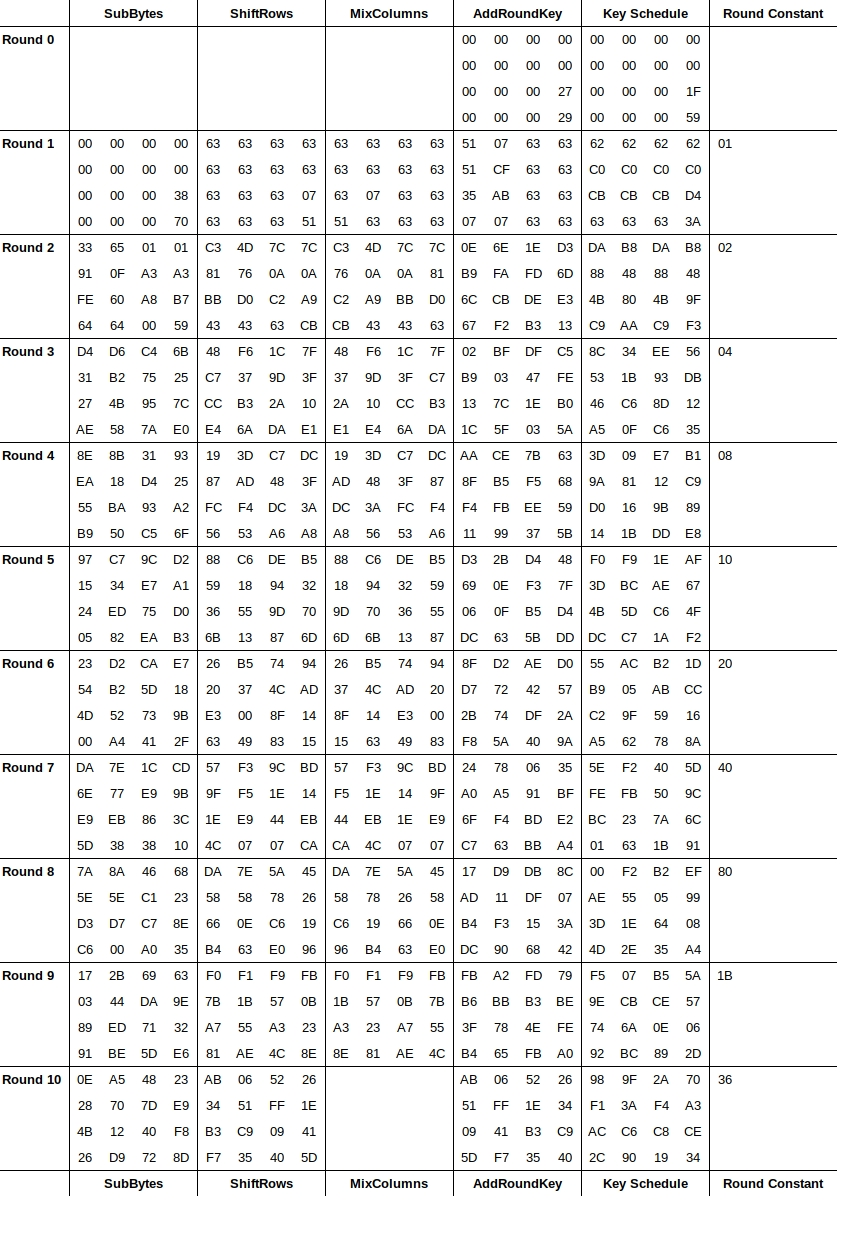
\includegraphics[width=1\linewidth]{imgs/table_aes_deph.jpg}
    \caption{Tabela com 10 rounds de decifração.}
    \label{fig:tab2}
\end{figure}

\end{document}
